\section{ТЕОРЕТИЧЕСКИЕ СВЕДЕНИЯ}

\subsection{Набор регистров}

В программах на языке ассемблер регистры микропроцессора используются очень интенсивно.
Основные программно-доступные регистры изображены на рисунке~\ref{fig:registers}.

\begin{figure}[htbp]
  \centering
  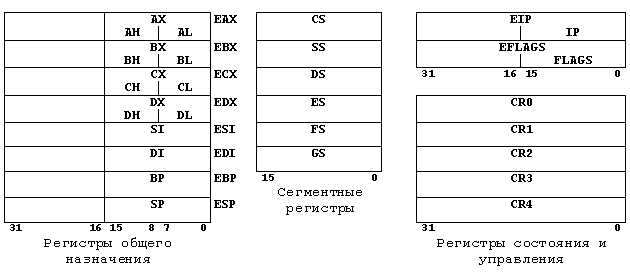
\includegraphics[width=150mm]{pic/registers}
  \caption{Основные регистры 32-разрядных процессоров}\label{fig:registers}
\end{figure}

\textbf{Регистры общего назначения} без каких-либо ограничений могут использоваться
для хранения операндов логических и арифметических операций, компонентов адреса, указателей
на ячейки памяти, однако, каждый из них имеет определенное функциональное назначение:

\begin{itemize}
\item EAX/AX/AH/AL (Accumulator register) --- аккумулятор --- применяется для хранения
  промежуточных данных, а также адресов;
\item EBX/BX/BH/BL (Base register) --- базовый регистр --- применяется для хранения
  промежуточных данных, а также для хранения базового адреса объектов в памяти;
\item ECX/CX/CH/CL (Count register) --- регистр-счетчик --- применяется для хранения
  промежуточных данных, а также в циклических командах, производящих некоторые
  повторяющиеся действия, в качестве счетчика итераций;
\item EDX/DX/DH/DL (Data register) --- регистр данных --- так же, как и регистр EAX/AX/AH/AL, он
  используется для хранения промежуточных данных.
\end{itemize}

\textbf{Сегментные регистры} предназначены для аппаратной поддержки структурной
организации программы в виде отдельных частей, называемых сегментами.
Сегмент представляет собой независимый блок памяти фиксированного размера.
Операционная система размещает сегменты программы в оперативной памяти,
после чего помещает их адреса в соответствующие сегментные регистры.

Микропроцессор поддерживает следующие типы сегментов:

\begin{itemize}
\item сегмент кода --- содержит машинные команды, для доступа к нем у служит регистр CS
  (Code Segment register) --- сегментный регистр кода;
\item сегмент стека --- для доступа к нему служит регистр SS (Stack Segment register) ---
  сегментный регистр стека;
\item сегмент данных --- содержит обрабатываемые программой данные, для доступа к нему
  служит регистр DS (Data Segment register) --- сегментный регистр данных;
\item
  дополнительные сегменты данных --- их адреса должны содержаться в регистрах ES, GS, FS.
\end{itemize}

\subsection{Типы данных}

Микропроцессор аппаратно поддерживает следующие основные типы данных:

\begin{itemize}
\item байт --- восемь последовательно расположенных битов;
\item слово --- два байта, имеющих последовательные адреса;
\item двойное слово --- четыре байта, расположенных по последовательным адресам;
\item учетверенное слово --- восемь байт, расположенных по последовательным адресам;
\item 128-разрядный упакованный тип данных --- появился в МП Pentium III;
\end{itemize}

\subsection{Структура программы}

Программа на языке ассемблер состоит из строк, содержащих следующие поля:

метка: команда/директива операнды ;комментарий

Все эти поля в отдельных случаях необязательны. Метка, как и все идентификаторы в
программе, может быть любой комбинацией символов английского алфавита, цифр и символов
<<\_>>, <<\$>>, <<@>>, <<?>>. Цифра не может быть первым символом метки или идентификатора. 
В поле команды может располагаться команда процессора, которая будет транслирована в 
исполнимый код, или директива, которая не приводит к генерации кода, а управляет работой
самого транслятора (ассемблера). В поле операндов располагаются требуемые командой или
директивой операнды. Текст от символа <<;>> транслятором не анализируется и используется
в качестве комментария.

\subsection{Директивы распределения памяти}

Определение переменных (выделение памяти для переменных в коде программы) в общем
виде записывается следующим образом:

name d* value

где d* --- одна из псевдокоманд: db --- определить байт, dw --- определить слово (2 байта), dd ---
определить двойное слово (4 байта), df или dp --- определить 6 байт (дальний указатель), dq ---
определить учетверенное слово (8 байт), dt --- определить 10 байт (80-битные типы данных,
используемые FPU).

\subsection{Формат команд и режимы адресации}

В машинную команду микропроцессора явно или неявно входят следующие элементы:

\begin{itemize}
\item поле префиксов --- элемент команды, который уточняет либо модифицирует действие этой
  команды;
\item поле кода операции, определяющее действие данной команды;
\item поле операндов; содержит от 0 до 3 элементов.
\end{itemize}

Важной особенностью машинных команд является то, что они не могут манипулировать
одновременно двумя операндами, находящимися в оперативной памяти. По этой причине
возможны только следующие сочетания операндов в команде:

\begin{itemize}
\item регистр - регистр;
\item регистр - память;
\item память - регистр;
\item регистр - непосредственный операнд;
\item память - непосредственный операнд.
\end{itemize}

Из перечисленных сочетаний операндов наиболее часто употребляются регистр - память и
память - регистр.

Рассмотрим режимы адресации:
Прямая адресация --- простейший вид адресации операнда в памяти.

Прямая адресация может быть двух типов:
\begin{itemize}
\item относительная --- используется в командах условного и безусловного перехода;
\item абсолютная --- используется редко.
\end{itemize}